\documentclass[12pt]{article}
\usepackage[french]{babel}
\usepackage[T1]{fontenc}
\usepackage{listings}
\usepackage{amsmath,amsthm,amssymb,amsfonts}
\usepackage[dvipsnames]{xcolor}
\usepackage{pgfpages}
\usepackage{fullpage}
\usepackage[unicode,psdextra]{hyperref}
\usepackage{graphics}
\usepackage{float}
\usepackage{fancyvrb}

%---------------------------------------%
%             Paramétrage               %
%---------------------------------------%

\lstloadlanguages{C, Caml, Python, SQL}
\lstdefinestyle{CustomCodeBlock}{
    backgroundcolor = \color{gray!10!white},   
    commentstyle = \color{OliveGreen},
    identifierstyle=\color{Tan},
    keywordstyle = \color{MidnightBlue},
    numberstyle = \tiny \color{Gray},
    stringstyle = \color{Orchid},
    basicstyle = \ttfamily \footnotesize,
    breakatwhitespace = false,         
    breaklines = false,                 
    captionpos = b,                    
    keepspaces = false,                 
    numbers = left,                    
    numbersep = 5pt,                  
    showspaces = false,                
    showstringspaces = false,
    showtabs = false,                  
    tabsize = 3,
}
\lstset{style = CustomCodeBlock}



\hypersetup{
	colorlinks,
	citecolor=black,
	filecolor=black,
	linkcolor=black,
	urlcolor=black
}

%---------------------------------------%
%         Information  Générale         %
%---------------------------------------%

\title{Rapport de projet\\ Platformer}
\author{\small FARGEAT Alexis, MAGNIN Mathis, VERDIER Vincent}

%---------------------------------------%
%                Document               %
%---------------------------------------%

\begin{document}

	\maketitle

	\begin{figure}[H]
		\centering
		\begin{BVerbatim}
 _____  ______                               
|  __ \|  ____|                             
| |__) | |__ ___  _ __ _ __ ___   ___ _ __   
|  ___/|  __/ _ \| '__| '_ ` _ \ / _ | '__|
| |    | | | (_) | |  | | | | | |  __| |     
|_|    |_|  \___/|_|  |_| |_| |_|\___|_|   


		\end{BVerbatim}
	\end{figure}

	\tableofcontents
	\newpage

	\section{Introduction}
	
		\begin{center}
			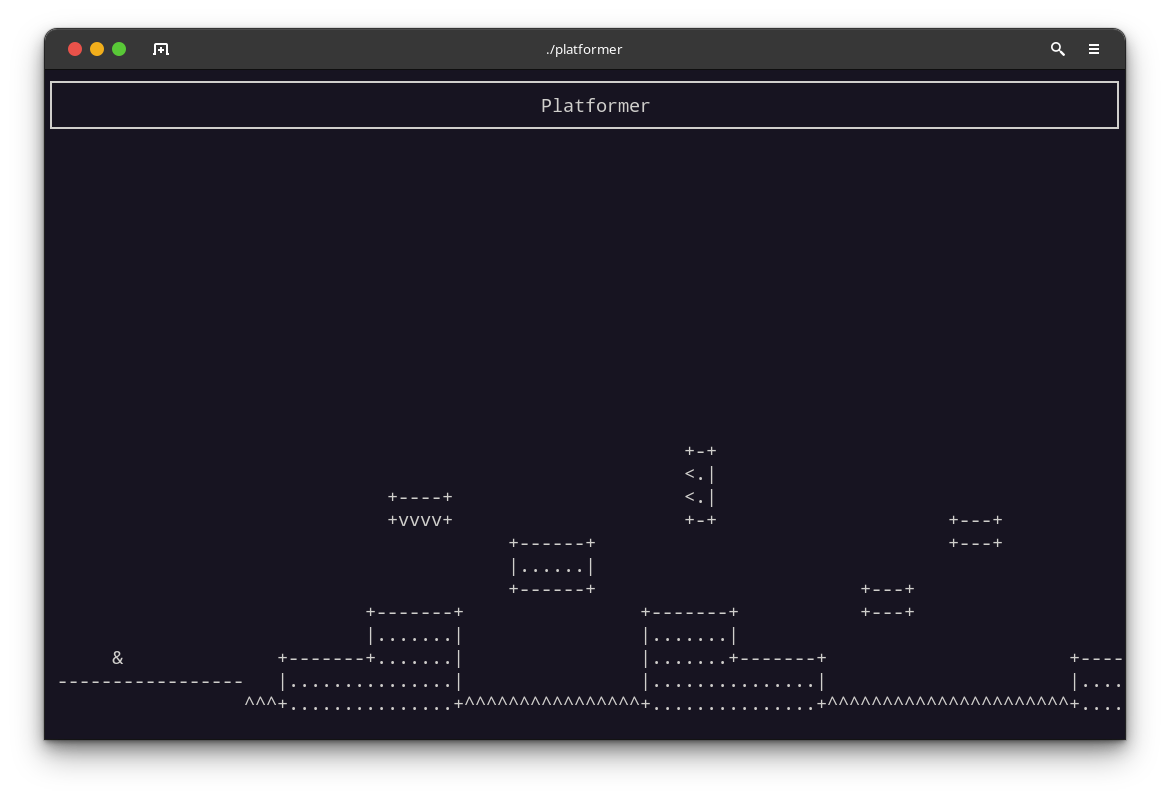
\includegraphics[width=0.90\textwidth]{content/image.png}
		\end{center}
	
		Platformer est un jeu de plateforme, où le but est d'arriver au bout d'une carte après de multiple obstacles.
		Ce jeu se rapproche de Mario Bros.
	
		Le jeu est programmé en \textbf{C} et s'utilise dans une console (similaire a MS-DOS).\\

		Le jeu est séparé en 4 grandes parties :
		\begin{itemize}
			\item map : Gestion du chargement et de la création de la carte
			\item affichage : Gestion de l'affichage et des différents menus et du jeu
			\item gameplay : Gestion du mouvement, des collisions, \dots
			\item moteur : Gestion des calculs internes\\
		\end{itemize}
	
	\newpage

	\section{Problèmes rencontrés}

		\subsection{Chargement de la carte}
		
			Au cours de la création du jeu, il a fallu choisir une manière de stocker les données de la carte du jeu.\\


			Nous cherchions une solution permettant un accès simple par les autres parties du programme comme l’affichage.
		
			Nous voulions également avoir la possibilité de modifier la carte du jeu de manière visuelle et sans recompiler le jeu.\\


			Cela nous a amené à choisir de stocker la carte dans un fichier texte qui sera chargé dans le jeu sous forme 
			d’un tableau à deux dimensions de taille dynamique.\\
		
			Au lancement du jeu, les données du fichier texte sont lues et la taille du tableau à allouer est calculée en 
			comptant le nombre de caractères de la ligne du haut de la carte.\\
		
			On stocke alors dans une structure  :
			\begin{itemize}
				\item Les dimensions \((x, y)\) de la carte
				\item Un tableau contenant les données du fichier texte
				\item Un autre tableau utile pour les collisions dont le fonctionnement est détaillé dans la partie Collisions.
			\end{itemize}
		
			Un tableau en \(2D\) de taille dynamique nécessite de libérer la mémoire occupée celui-ci l’arrêt du programme.
		
			Un tableau en \(2D\) peut être vu comme un tableau en \(1D\) stockant des pointeurs qui pointent le premier élément 
			de chaque colonne. Ce tableau en \(1D\) correspond à la première ligne du tableau en \(2D\).
		
			Pour libérer la mémoire occupée par le tableau on libère d’abord la mémoire occupée par chaque colonne puis 
			on libère la mémoire occupée par la première ligne.
			
		\newpage
		
	
		\subsection{Physique et mouvement}
		
		Le mouvement du joueur est modélisé grâce aux équations horaires du mouvement en physique
		
		\subsubsection{Sous-structures nécessaire pour l'implémentation}
		
		Cependant, pour il faut d'abord créer un moyen de compter le temps : le compter en secondes directement aurait été compliqué et peu précis, nous avons donc intégrer un compteur d'image qui est incrémenté à chaque passage dans la boucle principale.
		
		\medskip
		
		Ainsi, pour faciliter les modifications de valeurs, on utilise deux structure : \textit{vecteur} et \textit{coords}.
		Ces structures sont composés de deux variable \(x\) et \(y\)(qui décomposent le mouvement sur les deux axes), en flottant pour \textit{vecteur} et entier pour \textit{coords}. Ces deux types ont été nécessaire car lors d'un mouvement les coordonnées changent de très peu, ce qui ne pourrait pas être stocké convenablement dans des entiers, et la position du joueur ne peut être que entière.  
		
		Un autre type, \textit{mouvement} est utilisé pour stocker les actions en cours sur le joueur. La solution retenue ici à été de créer une variable de mouvement pour la vitesse et l'accélération mais en décomposant le mouvement en \(x\) et \(y\). Cette structure mouvement contient une valeur flottante, mais également une horloge, qui indique l'image de départ du mouvement.
		 
		\medskip
		On a créé alors la structure joueur contenant toutes les structures présentées ci-dessus. (\textit{cf. gameplay/joueur.c})
		
		\subsubsection{Calcul de l'écart entre deux positions}
		
		La position du joueur est calculée grâce aux valeurs de vitesse et d'accéleration sur chaque axe ainsi que leur image (\textit{frame}) de départ.
		
		Pour calculer la position du joueur à une image \(n + 1\), on prend la position du joueur à l'image \(n\) et on ajoute le petit déplacement \(dx\) (ou \(dy\) selon l'axe).
		
		On définit donc \(p_x(t)\) (position du joueur sur \(x\) en fonction du temps) comme :
		\begin{align*}
			p_x(t+1) &= p_x(t) + dx\\
			p_x(t+1)&= p_x(t) + (a_x \times [(t+1)^2 - t^2] + v_x)
		\end{align*}		
	
		Avec \(t\) le temps depuis le début du mouvement en question (\(t = \text{Image actuelle} - \text{tempsModification}\)).
		
		On calcule l'écart de position dû à l'accélération en faisant \((t+1)^2 - t^2\) car l'accélération est quadratique pour la position (on intègre deux fois une constante).
		
		Pour l'écart de la position dû à la vitesse, cette formule n'est pas nécessaire car la vitesse n'est intégré qu'une fois pour obtenir la position, donc est linéaire. Ainsi, à chaque incrémentation du temps, on ajoute la vitesse multipliée par \((t + 1) - t = 1\).
		
		De même pour le mouvement sur y.
		
		\subsubsection{Changement de la position du joueur}
		
		Une fois l'écart entre deux positions successives, on ajoute la valeur de cet écart (qui est un flottant) à la partie \textit{positionPrécise} de la structure du joueur. 
		
		Ensuite, comme pour l'affichage la position du joueur est interprété en entier, on utilise la fonction \(round\) qui arrondi la valeur à l'entier le plus proche.
		
		On stocke enfin cette valeur arrondie dans la partie \textit{position} de la structure joueur.
		
		\newpage
		
		\subsection{Affichage}
		
			L'affichage et une part importante d'un jeu, elle est la première interaction d'un joueur avec celui-ci.\\


			Le problème c'est posé lorsqu'il a fallu afficher la carte en fonction de la position du joueur dans celle-ci.

			En effet, Il est important qu'un joueur puisse voir suffisamment ce qui l'entoure afin d'avoir une bonne expérience de jeu.

			Nous avons donc opté sur la mise en place d'une \textit{camera} via l'implémentation d'une structure.
			\begin{lstlisting}[title=Structure Camera]
typedef struct s_camera {
	
	int centrex;
	int centrey;
	int longueur;
	int largeur;
				
} camera;
			\end{lstlisting}

		\subsection{Collisions}
		
		
		

	\section{Conclusion}

	Parmi les idées qui auraient pû améliorer le jeu, nous avons retenu :
	\begin{itemize}
		\item Un menu pour choisir différentes cartes
		\item Des adversaires automatiques
		\item Des couleurs
		\item Éventuellement, un outil pour créer d'autres cartes (ou un guide)
		\item \dots
	\end{itemize}
		
\end{document}